\documentclass{beamer}\usepackage[]{graphicx}\usepackage[]{color}
%% maxwidth is the original width if it is less than linewidth
%% otherwise use linewidth (to make sure the graphics do not exceed the margin)
\makeatletter
\def\maxwidth{ %
  \ifdim\Gin@nat@width>\linewidth
    \linewidth
  \else
    \Gin@nat@width
  \fi
}
\makeatother

\definecolor{fgcolor}{rgb}{0.345, 0.345, 0.345}
\newcommand{\hlnum}[1]{\textcolor[rgb]{0.686,0.059,0.569}{#1}}%
\newcommand{\hlstr}[1]{\textcolor[rgb]{0.192,0.494,0.8}{#1}}%
\newcommand{\hlcom}[1]{\textcolor[rgb]{0.678,0.584,0.686}{\textit{#1}}}%
\newcommand{\hlopt}[1]{\textcolor[rgb]{0,0,0}{#1}}%
\newcommand{\hlstd}[1]{\textcolor[rgb]{0.345,0.345,0.345}{#1}}%
\newcommand{\hlkwa}[1]{\textcolor[rgb]{0.161,0.373,0.58}{\textbf{#1}}}%
\newcommand{\hlkwb}[1]{\textcolor[rgb]{0.69,0.353,0.396}{#1}}%
\newcommand{\hlkwc}[1]{\textcolor[rgb]{0.333,0.667,0.333}{#1}}%
\newcommand{\hlkwd}[1]{\textcolor[rgb]{0.737,0.353,0.396}{\textbf{#1}}}%

\usepackage{framed}
\makeatletter
\newenvironment{kframe}{%
 \def\at@end@of@kframe{}%
 \ifinner\ifhmode%
  \def\at@end@of@kframe{\end{minipage}}%
  \begin{minipage}{\columnwidth}%
 \fi\fi%
 \def\FrameCommand##1{\hskip\@totalleftmargin \hskip-\fboxsep
 \colorbox{shadecolor}{##1}\hskip-\fboxsep
     % There is no \\@totalrightmargin, so:
     \hskip-\linewidth \hskip-\@totalleftmargin \hskip\columnwidth}%
 \MakeFramed {\advance\hsize-\width
   \@totalleftmargin\z@ \linewidth\hsize
   \@setminipage}}%
 {\par\unskip\endMakeFramed%
 \at@end@of@kframe}
\makeatother

\definecolor{shadecolor}{rgb}{.97, .97, .97}
\definecolor{messagecolor}{rgb}{0, 0, 0}
\definecolor{warningcolor}{rgb}{1, 0, 1}
\definecolor{errorcolor}{rgb}{1, 0, 0}
\newenvironment{knitrout}{}{} % an empty environment to be redefined in TeX

\usepackage{alltt} 
% \usepackage{graphicx}
\usepackage{graphics}
\usepackage[T1]{fontenc}
\usepackage{hyperref}
\setbeamercovered{transparent}
\renewcommand{\ni}{\noindent}
\hypersetup{
  colorlinks   = true, %Colours links instead of ugly boxes
  urlcolor     = blue, %Colour for external hyperlinks
  linkcolor    = blue, %Colour of internal links
  citecolor   = red %Colour of citations
}
%load packages that will be invisible on slides


\title[Advanced Graphics in R]{2 - Advanced Graphics in R}
\subtitle{03 - Plotting Using Layers}
\author[ ]{}
\date{\hspace{1in}}
\institute[ISU]{Iowa State University}
\IfFileExists{upquote.sty}{\usepackage{upquote}}{}
\begin{document}

\begin{frame}
    \maketitle
\end{frame}

%-----------------------------------------------------------------------------

\begin{frame}
\frametitle{Outline}
\begin{itemize}
    \item Data Sources
    \item Layers
    \item \texttt{ggplot()} vs. \texttt{qplot()}
\end{itemize}    
\end{frame}



%-----------------------------------------------------------------------------

\begin{frame}[fragile]
\frametitle{Deepwater Horizon Oil Spill}

\begin{figure}[hbtp]\centering
\includegraphics[keepaspectratio=true, width=.85\linewidth]{figure/satelitepicBPoilspill.png}
\end{figure}

\end{frame}


%-----------------------------------------------------------------------------

\begin{frame}
\frametitle{Data Sets}

NOAA Data
\begin{itemize}
    \item National Oceanic and Atmospheric Administration
    \item Temperature and Salinity Data in Gulf of Mexico
    \item Measured using Floats, Gliders and Boats
\end{itemize} 
\medskip
US Fisheries and Wildlife Data
\begin{itemize}
    \item Animal Sightings on the Gulf Coast
    \item Birds, Turtles and Mammals
    \item Status: Oil Covered or Not
\end{itemize} 
Both data sets have geographic coordinates for ever observation
\end{frame}

%-----------------------------------------------------------------------------

\begin{frame}[fragile]
\frametitle{Loading NOAA Data}
NOAA data is a \texttt{.rdata} file so we need to read it in specially
   \begin{itemize}
    \item Download the data from {\small\url{http://www.public.iastate.edu/~hofmann/looking-at-data/data/noaa.rdata}}
    \item Save the noaa data file from the website to your working directory folder
    \item To figure out your working directory location use \texttt{getwd()}
    \item Then use the code below to load the data into R
\end{itemize} 
\small
\begin{knitrout}\footnotesize
\definecolor{shadecolor}{rgb}{1, 1, 1}\color{fgcolor}\begin{kframe}
\begin{alltt}
  \hlkwd{setwd}\hlstd{(}\hlstr{" - your WD location here - "}\hlstd{)}
  \hlkwd{load}\hlstd{(}\hlstr{"noaa.rdata"}\hlstd{)}
\end{alltt}
\end{kframe}
\end{knitrout}
\vspace{-25pt}
\begin{knitrout}\footnotesize
\definecolor{shadecolor}{rgb}{1, 1, 1}\color{fgcolor}\begin{kframe}
\begin{alltt}
\hlkwd{options}\hlstd{(}\hlkwc{width}\hlstd{=}\hlnum{65}\hlstd{)}
  \hlkwd{ls}\hlstd{()}
\end{alltt}
\begin{verbatim}
## [1] "animals" "boats"   "floats"  "gliders" "rig"     "states"
\end{verbatim}
\end{kframe}
\end{knitrout}
    \normalsize
\end{frame}


%-----------------------------------------------------------------------------

\begin{frame}[fragile]
\frametitle{Floats}
Lets take a peek at the top of the floats NOAA data.

\small
\begin{knitrout}\footnotesize
\definecolor{shadecolor}{rgb}{1, 1, 1}\color{fgcolor}\begin{kframe}
\begin{verbatim}
##   callSign Date_Time JulianDay Time_QC Latitude
## 1 Q4901043 7/12/2010   2455390       1    24.82
## 2 Q4901043 7/12/2010   2455390       1    24.82
## 3 Q4901043 7/12/2010   2455390       1    24.82
##   Longitude Position_QC Depth Depth_QC Temperature
## 1    -87.96           1     2        1       29.83
## 2    -87.96           1     4        1       29.65
## 3    -87.96           1     6        1       29.53
##   Temperature_QC Salinity Salinity_QC  Type
## 1              1    36.59           1 Float
## 2              1    36.58           1 Float
## 3              1    36.58           1 Float
\end{verbatim}
\end{kframe}
\end{knitrout}
    \normalsize
\end{frame}


%-----------------------------------------------------------------------------

\begin{frame}[fragile]
\frametitle{Floats}

\begin{knitrout}\footnotesize
\definecolor{shadecolor}{rgb}{1, 1, 1}\color{fgcolor}

{\centering 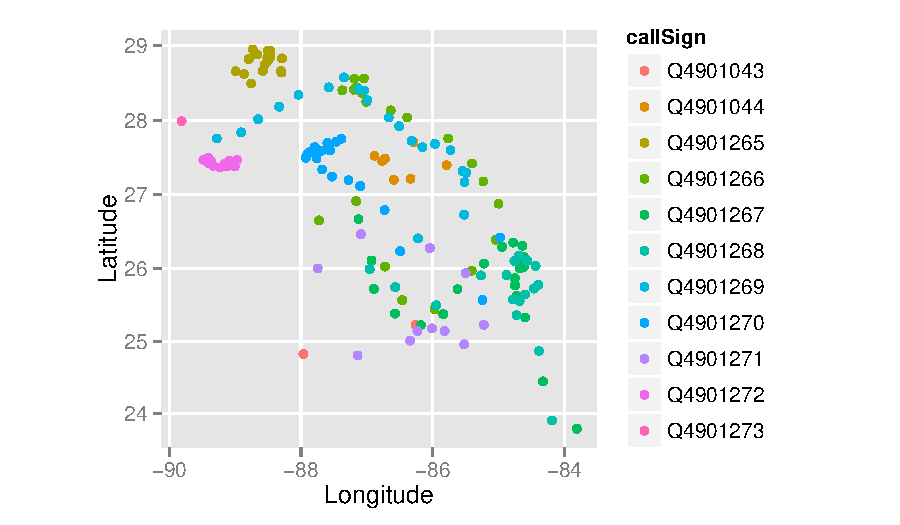
\includegraphics[width=.9\linewidth]{figure/kfloats2} 

}



\end{knitrout}

\end{frame}

%-----------------------------------------------------------------------------

\begin{frame}[fragile]
\frametitle{Gliders}

\begin{knitrout}\footnotesize
\definecolor{shadecolor}{rgb}{1, 1, 1}\color{fgcolor}

{\centering \includegraphics[width=.9\linewidth]{figure/gliders} 

}



\end{knitrout}
\end{frame}


%-----------------------------------------------------------------------------

\begin{frame}[fragile]
\frametitle{Boats}

\begin{knitrout}\footnotesize
\definecolor{shadecolor}{rgb}{1, 1, 1}\color{fgcolor}

{\centering \includegraphics[width=.9\linewidth]{figure/Boats} 

}



\end{knitrout}

\end{frame}

%-----------------------------------------------------------------------------

\begin{frame}[fragile]
\frametitle{Layering}
This data has the same context - a common time and common place

   \begin{itemize}
    \item Want to aggregate information from different sources onto a common plot\medskip
    \item Start with a common background the lat/long grid\medskip
    \item With \texttt{ggplot2} we will superimpose data onto this grid in layers\medskip
\end{itemize} 
\small

    \normalsize
\end{frame}


%-----------------------------------------------------------------------------

\begin{frame}[fragile]
\frametitle{Layers}
\vspace{-14pt}\hfill... to give you an idea ... \vspace{-9pt}
\begin{knitrout}\scriptsize
\definecolor{shadecolor}{rgb}{1, 1, 1}\color{fgcolor}\begin{kframe}
\begin{alltt}
\hlkwd{ggplot}\hlstd{()} \hlopt{+}   \hlcom{# plot without a default data set}
\hlkwd{geom_path}\hlstd{(}\hlkwc{data}\hlstd{=states,} \hlkwd{aes}\hlstd{(}\hlkwc{x}\hlstd{=long,} \hlkwc{y}\hlstd{=lat,} \hlkwc{group}\hlstd{=group))} \hlopt{+}
\hlkwd{geom_point}\hlstd{(}\hlkwc{data}\hlstd{=floats,} \hlkwd{aes}\hlstd{(}\hlkwc{x}\hlstd{=Longitude,} \hlkwc{y}\hlstd{=Latitude,} \hlkwc{colour}\hlstd{=callSign))} \hlopt{+}
\hlkwd{geom_point}\hlstd{(}\hlkwd{aes}\hlstd{(x, y),} \hlkwc{shape}\hlstd{=}\hlstr{"x"}\hlstd{,} \hlkwc{size}\hlstd{=}\hlnum{5}\hlstd{,} \hlkwc{data}\hlstd{=rig)} \hlopt{+}
\hlkwd{geom_text}\hlstd{(}\hlkwd{aes}\hlstd{(x, y),} \hlkwc{label}\hlstd{=}\hlstr{"BP Oil rig"}\hlstd{,} \hlkwc{shape}\hlstd{=}\hlstr{"x"}\hlstd{,}
          \hlkwc{size}\hlstd{=}\hlnum{5}\hlstd{,} \hlkwc{data}\hlstd{=rig,} \hlkwc{hjust} \hlstd{=} \hlopt{-}\hlnum{0.1}\hlstd{)} \hlopt{+}
\hlkwd{xlim}\hlstd{(}\hlkwd{c}\hlstd{(}\hlopt{-}\hlnum{91}\hlstd{,} \hlopt{-}\hlnum{80}\hlstd{))} \hlopt{+} \hlkwd{ylim}\hlstd{(}\hlkwd{c}\hlstd{(}\hlnum{22}\hlstd{,}\hlnum{32}\hlstd{))} \hlopt{+} \hlkwd{coord_map}\hlstd{()}
\end{alltt}
\end{kframe}

{\centering \includegraphics[width=.9\linewidth]{figure/layers1} 

}



\end{knitrout}

\end{frame}

%-----------------------------------------------------------------------------

\begin{frame}[fragile]
\frametitle{Layering}
   \begin{itemize}
    \item Most maps (and many plots) have multiple layers of data. The layers may be from the same or different datasets.\bigskip
    \item ggplot2 build around this same idea. Very easy to add additional layers to the plot. To do this we need to understand a little more about the underlying theory.
\end{itemize} 
\small

    \normalsize
\end{frame}

%-----------------------------------------------------------------------------

\begin{frame}[fragile]
\frametitle{What is a Plot?}
    Any plot is composed of:
   \begin{enumerate}
    \item A default dataset 
    \item A coordinate system
    \item layers of geometric objects (geoms)
    \item A set of aesthetic mappings (taking information from the data and converting into an attribute of the plot)
    \item A scale for each aesthetic
    \item A facetting specification (multiple plots based on subsetting the data)
\end{enumerate} 
\end{frame}

%-----------------------------------------------------------------------------

\begin{frame}[fragile]
\frametitle{Floats Decomposed}
\begin{minipage}{.35\linewidth}
\textbf{Data:} floats \\
\textbf{Mappings:}
\footnotesize

\begin{tabular}{rcl}
x&=&Longitude \\
y&=&Latitude\\
color&=&CallSign\\
\end{tabular}\normalsize

\textbf{Layers:} 
\footnotesize

\begin{tabular}{rl}
Geoms: & Points\\
\end{tabular}
\normalsize

\textbf{Scales:} 
\footnotesize

\begin{tabular}{l}
x \& y position\\
discrete color
\end{tabular}
\normalsize

\textbf{Faceting:} None
\end{minipage}
\begin{minipage}{.6\linewidth}\centering
\includegraphics[keepaspectratio=TRUE,width=.92\linewidth]{figure/kfloats3}
\end{minipage}
\end{frame}

%-----------------------------------------------------------------------------

\begin{frame}[fragile]
\frametitle{\texttt{qplot()} vs. \texttt{ggplot()}}
\texttt{qplot()} stands for ``quickplot'' \medskip
\begin{itemize}
  \item automatically chooses default settings to make life easier\medskip
  \item less control over plot construction\bigskip
\end{itemize} 
    
\texttt{ggplot()} stands for ``grammar of graphics plot'' \medskip
\begin{itemize}
  \item Constructs the plot using components listed in previous slides
\end{itemize} 
\end{frame}


%-----------------------------------------------------------------------------

\begin{frame}[fragile]
\frametitle{\texttt{qplot()} vs. \texttt{ggplot()}}
Two ways to construct the same plot for float locations 
\begin{knitrout}\footnotesize
\definecolor{shadecolor}{rgb}{1, 1, 1}\color{fgcolor}\begin{kframe}
\begin{alltt}
\hlkwd{qplot}\hlstd{(Longitude, Latitude,} \hlkwc{colour}\hlstd{=callSign,} \hlkwc{data}\hlstd{=floats)}

\hlcom{###}

\hlkwd{ggplot}\hlstd{(}\hlkwc{data}\hlstd{=floats,}
       \hlkwd{aes}\hlstd{(}\hlkwc{x}\hlstd{=Longitude,} \hlkwc{y}\hlstd{=Latitude,} \hlkwc{colour}\hlstd{=callSign))} \hlopt{+}
  \hlkwd{geom_point}\hlstd{()} \hlopt{+}
  \hlkwd{scale_x_continuous}\hlstd{()} \hlopt{+}
  \hlkwd{scale_y_continuous}\hlstd{()} \hlopt{+}
  \hlkwd{scale_colour_discrete} \hlstd{()}

\hlcom{###}

\hlcom{# But we don't need to be quite so verbose.  Scales are}
\hlcom{# added automatically and first two aes params are x and y:}
\hlkwd{ggplot}\hlstd{(floats,}
       \hlkwd{aes}\hlstd{(Longitude, Latitude,} \hlkwc{colour} \hlstd{= callSign))} \hlopt{+}
  \hlkwd{geom_point}\hlstd{()}
\end{alltt}
\end{kframe}
\end{knitrout}
\end{frame}


%-----------------------------------------------------------------------------
\begin{frame}[fragile]
\frametitle{Floats Decomposed}
\begin{minipage}{.35\linewidth}
\textbf{Data:} floats \\
\textbf{Mappings:}
\footnotesize

\begin{tabular}{rcl}
x&=&Longitude \\
y&=&Latitude\\
color&=&CallSign\\
\end{tabular}\normalsize

\textbf{Layers:} 
\footnotesize

\begin{tabular}{rl}
Geoms: & Points\\
\end{tabular}
\normalsize

\textbf{Scales:} 
\footnotesize

\begin{tabular}{l}
x \& y position\\
discrete color
\end{tabular}
\normalsize

\textbf{Faceting:} None
\end{minipage}
\begin{minipage}{.6\linewidth}\centering
\includegraphics[keepaspectratio=TRUE,width=.92\linewidth]{figure/kfloats3}
\end{minipage}
\end{frame}


%-----------------------------------------------------------------------------

\begin{frame}[fragile]
\frametitle{\texttt{qplot()} vs. \texttt{ggplot()}}
\begin{minipage}{.37\linewidth}
\textbf{Data:} floats \\
\textbf{Mappings:}
\footnotesize

\begin{tabular}{rcl}
x&=&CallSign \\
y&=&Temperature\\
\end{tabular}\normalsize

\textbf{Layers:} 
\footnotesize

\begin{tabular}{rl}
Geoms: & Jittered Points\\
& Boxplots
\end{tabular}
\normalsize

\textbf{Scales:} 
\footnotesize

\begin{tabular}{l}
x \& y position
\end{tabular}
\normalsize

\textbf{Faceting:} None
\end{minipage}
\begin{minipage}{.6\linewidth}\centering
\includegraphics[keepaspectratio=TRUE,width=.92\linewidth]{figure/qvsgg2}
\end{minipage}
\end{frame}

%-----------------------------------------------------------------------------

\begin{frame}[fragile]
\frametitle{\texttt{qplot()} vs. \texttt{ggplot()}}
Again, there are two ways to construct this plot 
\begin{knitrout}\footnotesize
\definecolor{shadecolor}{rgb}{1, 1, 1}\color{fgcolor}\begin{kframe}
\begin{alltt}
\hlcom{# Temperature by callSign}
\hlcom{### using qplot}
\hlkwd{qplot}\hlstd{(callSign, Temperature,} \hlkwc{data}\hlstd{=floats,}
      \hlkwc{geom}\hlstd{=}\hlkwd{c}\hlstd{(}\hlstr{"jitter"}\hlstd{,} \hlstr{"boxplot"}\hlstd{))}

\hlcom{### using ggplot}
\hlkwd{ggplot}\hlstd{(floats,} \hlkwd{aes}\hlstd{(callSign, Temperature))} \hlopt{+}
  \hlkwd{geom_jitter}\hlstd{()} \hlopt{+}
  \hlkwd{geom_boxplot}\hlstd{()}
\end{alltt}
\end{kframe}
\end{knitrout}
\end{frame}

%-----------------------------------------------------------------------------

\begin{frame}[fragile]
\frametitle{Your Turn}
Find the \texttt{ggplot()} statement that creates this plot
\begin{knitrout}\footnotesize
\definecolor{shadecolor}{rgb}{1, 1, 1}\color{fgcolor}

{\centering \includegraphics[width=.9\linewidth]{figure/ggyourturn} 

}



\end{knitrout}
\end{frame}

%-----------------------------------------------------------------------------

\begin{frame}
\frametitle{What is a layer?}
    A layer added to \texttt{ggplot()} can be a geom ...
\begin{itemize}
  \item the type of geometric object
  \item the statistic mapped to that object
  \item the data set from which to obtain the statistic
\end{itemize}
    \vspace{.25in}
    ... or a position adjustment to the scales
\begin{itemize}
  \item Changing the axes scale
  \item Changing the color gradient
\end{itemize}
    
\end{frame}


%-----------------------------------------------------------------------------

\begin{frame}
\frametitle{Layer Examples}

\begin{table}[ht]
\centering
\begin{tabular}{|l|ll|}
  \hline
Plot & Geom & Stat \\ 
  \hline
Scatterplot  & point  &  identity \\
Histogram  & bar  & bin count \\
Smoother  & line + ribbon & smoother function \\
Binned Scatterplot  & rectangle + color & 2d bin count \\
   \hline
\end{tabular}
\end{table}
    
More geoms described at \url{http://docs.ggplot2.org/current/}
\end{frame}

%-----------------------------------------------------------------------------

\begin{frame}[fragile]
\frametitle{Piecing things together}

Want to build a map using NOAA data
\begin{itemize}
  \item Coordinate system (mapping Long-Lat to X-Y)
  \item Add layer of state outlines
  \item Add layer of points for float locations
  \item Add layers for Oil Rig marker and label
  \item Adjust the range of x and y scales
\end{itemize}

\begin{knitrout}\footnotesize
\definecolor{shadecolor}{rgb}{1, 1, 1}\color{fgcolor}\begin{kframe}
\begin{alltt}
\hlkwd{ggplot}\hlstd{()} \hlopt{+}   \hlcom{# plot without a default data set}
 \hlkwd{geom_path}\hlstd{(}\hlkwc{data}\hlstd{=states,} \hlkwd{aes}\hlstd{(}\hlkwc{x}\hlstd{=long,} \hlkwc{y}\hlstd{=lat,} \hlkwc{group}\hlstd{=group))} \hlopt{+}
 \hlkwd{geom_point}\hlstd{(}\hlkwc{data}\hlstd{=floats,}
            \hlkwd{aes}\hlstd{(}\hlkwc{x}\hlstd{=Longitude,} \hlkwc{y}\hlstd{=Latitude,} \hlkwc{colour}\hlstd{=callSign))} \hlopt{+}
 \hlkwd{geom_point}\hlstd{(}\hlkwd{aes}\hlstd{(x, y),} \hlkwc{shape}\hlstd{=}\hlstr{"x"}\hlstd{,} \hlkwc{size}\hlstd{=}\hlnum{5}\hlstd{,} \hlkwc{data}\hlstd{=rig)} \hlopt{+}
 \hlkwd{geom_text}\hlstd{(}\hlkwd{aes}\hlstd{(x, y),} \hlkwc{label}\hlstd{=}\hlstr{"BP Oil rig"}\hlstd{,} \hlkwc{shape}\hlstd{=}\hlstr{"x"}\hlstd{,}
       \hlkwc{size}\hlstd{=}\hlnum{5}\hlstd{,} \hlkwc{data}\hlstd{=rig,} \hlkwc{hjust} \hlstd{=} \hlopt{-}\hlnum{0.1}\hlstd{)} \hlopt{+}
 \hlkwd{xlim}\hlstd{(}\hlkwd{c}\hlstd{(}\hlopt{-}\hlnum{91}\hlstd{,} \hlopt{-}\hlnum{80}\hlstd{))} \hlopt{+}
 \hlkwd{ylim}\hlstd{(}\hlkwd{c}\hlstd{(}\hlnum{22}\hlstd{,}\hlnum{32}\hlstd{))}
\end{alltt}
\end{kframe}
\end{knitrout}
\end{frame}


%-----------------------------------------------------------------------------

\begin{frame}[fragile]
\frametitle{Piecing things together}

\begin{knitrout}\footnotesize
\definecolor{shadecolor}{rgb}{1, 1, 1}\color{fgcolor}

{\centering \includegraphics[width=\linewidth]{figure/endmap2} 

}



\end{knitrout}
\end{frame}


%-----------------------------------------------------------------------------

\begin{frame}
\frametitle{Your Turn}
\begin{itemize}
  \item Read in the animal.csv data 
\bigskip
  \item Plot the location of animal sightings on a map of the region
  \item On this plot try to color points by class of animal and/or status of animal
\bigskip
  \item Advanced: Could we indicate time somehow?
\end{itemize}
\end{frame}

\end{document}
